\documentclass{article}
\usepackage{xeCJK}
\usepackage{amsmath}
\usepackage{listings}
\usepackage{xcolor}
\usepackage{float}
\setlength{\parindent}{0pt}
\renewcommand{\baselinestretch}{1.0}
\lstset{
	frame=tb, % draw a frame at the top and bottom of the code block
	showstringspaces=false, % don't mark spaces in strings
	numbers=left, % display line numbers on the left
	commentstyle=\color{green}, % comment color
	keywordstyle=\color{blue}, % keyword color
	stringstyle=\color{red} % string color
}
\usepackage[a4paper,left=20mm,right=20mm,top=15mm,bottom=15mm]{geometry}  

\title{find}
\author{MengChunlei}

\begin{document}
\maketitle
\section{基本用法}
$find$是用来在一个目录(包括子目录)下进行文件查找的命令,基本语法规则为:\par
\begin{center}
$find [paths] [expression] [actions]$
\end{center}
\begin{itemize}
	\item $paths$定义了查找的目录(可以是多个目录,用空格分隔)
	\item $expression$ 定义了查找文件的条件
	\item $action$定义了对于找到的文件要进行什么操作(打印出来,删除等等)
\end{itemize}
举个例子: $find ./ -name "*.txt" -print$ \par
\begin{itemize}
	\item $./$ 表示在当前目录及其子目录下进行查找
	\item $-name "*.txt"$ 表示查找名字后缀为$txt$的文件 
	\item $-print$ 表示对于找到的文件直接打印在屏幕上
\end{itemize}
\begin{figure}[h]
	\centering
	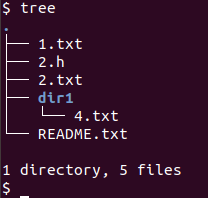
\includegraphics[scale=0.8]{pic1.png} \par
	\caption{当前目录结构}
\end{figure}

\begin{lstlisting}[language=bash]
$ find ./ -name "*.txt" -print
./2.txt
./README.txt
./dir1/4.txt
./1.txt
$ find ./ -name "*.txt"  /*默认的action为print*/
./2.txt
./README.txt
./dir1/4.txt
./1.txt
$ find  -name "*.txt" /*默认的paths为当前目录*/
./2.txt
./README.txt
./dir1/4.txt
./1.txt
$ find dir1/ dir2/  /*可以同时在多个目录中查找*/
dir1/
dir1/4.txt
dir2/
dir2/B.txt
dir2/dir
dir2/dir/README.txt
dir2/dir/B.TXT
dir2/dir/b.txt
dir2/a.txt
dir2/b.txt
$ find /tmp/ -name "*.log"
find: ‘/tmp/systemd-private-6ded1284157744119460 Permission denied
/tmp/XN4851.log
/tmp/hay4851.log
find: ‘/tmp/systemd-private-6ded128415774411946052051140cff6- Permission denied
find: ‘/tmp/systemd-private-6ded128415774411946052051140cff6-sys Permission denied
$ 
$ find /tmp/ -name "*.log" 2>/dev/null /*过滤错误*/
/tmp/XN4851.log
/tmp/hay4851.log
$ find /tmp/ -name ??????.log 2>/dev/null /*只搜索6个字符的log文件*/
/tmp/XN4851.log
\end{lstlisting}


\section{按照文件名字查找}
\begin{figure}[H]
	\centering
	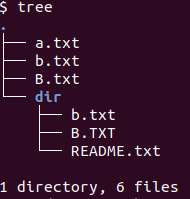
\includegraphics[scale=0.8]{pic2.png} \par
	\caption{当前目录结构}
\end{figure}

\begin{lstlisting}[language=bash]
$ find . -name b.txt
./dir/b.txt
./b.txt
$ find . -iname b.txt /*不区分大小写*/
./B.txt
./dir/B.TXT
./dir/b.txt
./b.txt
\end{lstlisting}

\section{按照文件大小查找}

\begin{lstlisting}[language=bash]
$ ll
total 32
drwxrwxr-x 2 nio nio 4096 4月  11 11:08 ./
drwxrwxr-x 5 nio nio 4096 4月  11 11:07 ../
-rw-rw-r-- 1 nio nio  119 4月  11 11:08 file1
-rw-rw-r-- 1 nio nio   35 4月  11 11:08 file2
-rw-rw-r-- 1 nio nio   54 4月  11 11:08 file3
-rw-rw-r-- 1 nio nio   31 4月  11 11:08 file4
-rw-rw-r-- 1 nio nio   23 4月  11 11:08 file5
-rw-rw-r-- 1 nio nio   10 4月  11 11:08 file6
$ find . -size -54c  /*小于54字节的文件*/
./file6
./file5
./file4
./file2
$ find . -size 54c /*等于54字节的文件*/
./file3
$ find . -size +54c /*大于54字节的文件*/
.
./file1
\end{lstlisting}
下面是文件单位: \par
\begin{itemize}
	\item $b$: 512字节的block
	\item $c$: 字节
	\item $k$: kb
	\item $M$: mb
	\item $G$: GB
\end{itemize}


\section{按照时间查找}
$Linux$中用到的时间有三种,访问时间(atime)、数据修改时间(mtime)、状态修改时间(ctime).平时常用的应该是$mtime$. 比如: \par

\begin{itemize}
	\item find . -mtime -5: 5天以内
	\item find . -mtime 5: 第五天
	\item find . -mtime +5: 6天前
\end{itemize}
下面是时间说明图:
\begin{figure}[H]
	\centering
	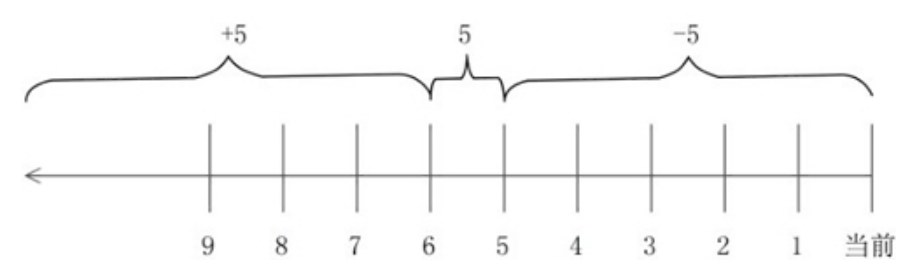
\includegraphics[scale=0.4]{pic3.png} \par
	\caption{时间说明图}
\end{figure}
另外,还有一组类似的以分钟作为单位的的命令: amin, mmin, cmin\par
还可以使用 -newer、-anewer 和 –cnewer 选项查找已修改或访问过的文件与特定的文件比较. \par
\begin{lstlisting}[language=bash]
$ echo aaa > 1.txt
$ echo bbb > 2.txt
$ echo ccc > 3.txt
$ find . -newer 2.txt  /*修改时间晚于2.txt的文件*/
.
./3.txt
\end{lstlisting}

\section{按照文件类型查找}
\begin{lstlisting}[language=bash]
$ ll
total 12
drwxrwxr-x 3 nio nio 4096 4月  11 11:00 ./
drwxrwxr-x 5 nio nio 4096 4月  11 11:07 ../
-rw-rw-r-- 1 nio nio    0 4月  11 10:59 a.txt
-rw-rw-r-- 1 nio nio    0 4月  11 10:59 b.txt
-rw-rw-r-- 1 nio nio    0 4月  11 11:00 B.txt
drwxrwxr-x 2 nio nio 4096 4月  11 11:00 dir/
$ find . -type f /*查找文件*/
./B.txt
./dir/README.txt
./dir/B.TXT
./dir/b.txt
./a.txt
./b.txt
$ find . -type d /*查找文件夹*/
.
./dir
\end{lstlisting}

\section{逻辑运算}
逻辑命令有三个,用来对条件做复合运算: \par
\begin{itemize}
	\item -a: 条件and
	\item -o: 条件或
	\item -not: 条件非
\end{itemize}
\begin{lstlisting}[language=bash]
$ find . -name b.txt -a -mmin -50 /*名字为b.txt且最近50分钟修改过的文件*/
./dir/b.txt
./b.txt
$ find . '(' -not -name b.txt ')' -o -type d /*名字不是b.txt或者文件夹*/
.
./B.txt
./dir
./dir/README.txt
./dir/B.TXT
./a.txt
\end{lstlisting}

\section{其他action}
$action$部分除了$print$以外还有两个命令: \par
\begin{itemize}
	\item -exec: 用来执行后面的命令
	\item -ok: 用来执行后面的命令,但是每次会询问是否执行
\end{itemize}
\begin{lstlisting}[language=bash]
$ ls
a.txt  b.txt  B.txt  dir
$ find . -name b.txt 
./dir/b.txt
./b.txt
$ 
$ find . -name b.txt -exec ls -l {} \;           /*对于每个找到的文件执行ls -l*/
-rw-rw-r-- 1 nio nio 0 4月  11 10:59 ./dir/b.txt /*其中{}织指代找到的文件*/
-rw-rw-r-- 1 nio nio 0 4月  11 10:59 ./b.txt
$ find . -name b.txt -exec rm {} \;  /*删掉找到的文件*/
$ ls
a.txt  B.txt  dir
$ find . -path "*/dir2/*.txt"
./dir5/dir2/a.txt
./dir5/dir/dir2/4.txt
./dir2/B.txt
./dir2/dir/README.txt
./dir2/dir/b.txt
./dir2/a.txt
./dir2/b.txt
$ find . -path "*/dir2/*.txt" -exec ls {} \; /*注意每找到一个打印一行*/
./dir5/dir2/a.txt
./dir5/dir/dir2/4.txt
./dir2/B.txt
./dir2/dir/README.txt
./dir2/dir/b.txt
./dir2/a.txt
./dir2/b.txt
$ find . -path "*/dir2/*.txt" -exec ls {} +  /*注意加号,所有的打印一行*/
./dir2/a.txt  ./dir2/b.txt  ./dir2/B.txt  ./dir2/dir/b.txt  ./dir2/dir/README.txt  ./dir5/dir2/a.txt  ./dir5/dir/dir2/4.txt
$ find . -path "*/dir2/*.txt" -exec tar -czvf dir_txt.gz {} + /*打包所有找到的文件*/
./dir5/dir2/a.txt
./dir5/dir/dir2/4.txt
./dir2/B.txt
./dir2/dir/README.txt
./dir2/dir/b.txt
./dir2/a.txt
./dir2/b.txt

\end{lstlisting}

\section{控制查找的深度}
\begin{figure}[H]
	\centering
	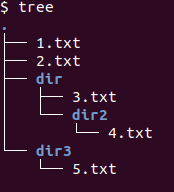
\includegraphics[scale=0.8]{pic4.png} \par
	\caption{时间说明图}
\end{figure}
\begin{lstlisting}[language=bash]
$ find .
.
./2.txt
./dir3
./dir3/5.txt
./1.txt
./dir
./dir/3.txt
./dir/dir2
./dir/dir2/4.txt
$ find . -maxdepth 1 /*只搜索深度为1的文件*/
.
./2.txt
./dir3
./1.txt
./dir
$ find . -mindepth 2 /*从深度为2开始搜索*/
./dir3/5.txt
./dir/3.txt
./dir/dir2
./dir/dir2/4.txt

\end{lstlisting}

\section{带路径搜索}
\begin{figure}[H]
	\centering
	
\includegraphics[scale=0.6]{pic5.png} \par
	\caption{时间说明图}
\end{figure}
\begin{lstlisting}[language=bash]
$ find . -path "*/dir2/*.txt" /*目标文件所在的文件夹为dir2*/
./dir5/dir2/a.txt
./dir5/dir/dir2/4.txt
./dir2/B.txt
./dir2/dir/README.txt
./dir2/dir/b.txt
./dir2/a.txt
./dir2/b.txt

\end{lstlisting}

\end{document}
